% Add the listed directories to the search path
% (allows easy moving of files around later)
% these paths are searched AFTER local config kpsewhich

% *.sty, *.cls
\makeatletter
\def\input@path{{@resources/texlive/texmf-local/tex/latex/}
        ,{@resources/texlive/texmf-local/bibtex/bst/},
        ,{@resources/texlive/texmf-local/bibtex/bib/},
        ,{@local/}
        }
\makeatother
\makeatletter
\def\bibinput@path{{@resources/texlive/texmf-local/tex/latex/}
        ,{@resources/texlive/texmf-local/bibtex/bst/},
        ,{@resources/texlive/texmf-local/bibtex/bib/},
        ,{@local/}
        }
\makeatother
  % allow latex to find custom stuff
% -*- mode: LaTeX; TeX-PDF-mode: t; -*- 
% LaTeX path to the root directory of the current project
% from the directory in which this file resides
% and path to econtexPaths which defines the rest of the paths like \FigDir
\providecommand{\econtexRoot}{}\renewcommand{\econtexRoot}{.}
\providecommand{\econtexPaths}{}\renewcommand{\econtexPaths}{econtexPaths}
% -*- mode: LaTeX; TeX-PDF-mode: t; -*- 
% The \commands below are required to allow sharing of the same base code via Github between TeXLive on a local machine and Overleaf (which is a proxy for "a standard distribution of LaTeX").  This is an ugly solution to the requirement that custom LaTeX packages be accessible, and that Overleaf prohibits symbolic links
\providecommand{\packages}{\econtexRoot/Resources/texmf-local/tex/latex}
\providecommand{\econtex}{\packages/econtex}
\providecommand{\econark}{\econtexRoot/Resources/texmf-local/tex/latex/econark}
\providecommand{\econtexSetup}{\econtexRoot/Resources/texmf-local/tex/latex/econtexSetup}
\providecommand{\econarkSetup}{\econtexRoot/Resources/texmf-local/tex/latex/econarkSetup}
\providecommand{\econtexShortcuts}{\econtexRoot/Resources/texmf-local/tex/latex/econtexShortcuts}
\providecommand{\econtexBibMake}{\econtexRoot/Resources/texmf-local/tex/latex/econtexBibMake}
\providecommand{\econtexBibStyle}{\econtexRoot/Resources/texmf-local/bibtex/bst/econtex}
\providecommand{\econtexBib}{economics}
\providecommand{\notes}{\econtexRoot/Resources/texmf-local/tex/latex/handout}
\providecommand{\handoutSetup}{\econtexRoot/Resources/texmf-local/tex/latex/handoutSetup}
\providecommand{\handoutShortcuts}{\econtexRoot/Resources/texmf-local/tex/latex/handoutShortcuts}
\providecommand{\handoutBibMake}{\econtexRoot/Resources/texmf-local/tex/latex/handoutBibMake}
\providecommand{\handoutBibStyle}{\econtexRoot/Resources/texmf-local/bibtex/bst/handout}

\providecommand{\FigDir}{\econtexRoot/Figures}
\providecommand{\CodeDir}{\econtexRoot/Code}
\providecommand{\DataDir}{\econtexRoot/Data}
\providecommand{\SlideDir}{\econtexRoot/Slides}
\providecommand{\TableDir}{\econtexRoot/Tables}
\providecommand{\ApndxDir}{\econtexRoot/Appendices}

\providecommand{\ResourcesDir}{\econtexRoot/Resources}
\providecommand{\rootFromOut}{..} % APFach back to root directory from output-directory
\providecommand{\LaTeXGenerated}{\econtexRoot/LaTeX} % Put generated files in subdirectory
\providecommand{\econtexPaths}{\econtexRoot/Resources/econtexPaths}
\providecommand{\LaTeXInputs}{\econtexRoot/Resources/LaTeXInputs}
\providecommand{\LtxDir}{LaTeX/}
\providecommand{\EqDir}{\econtexRoot/Equations} % Put generated files in subdirectory

\providecommand{\titlepagecustom}{\LaTeXInputs/titlepagecustom}


\documentclass[\econtexRoot/HAFiscal]{subfiles}

% \onlyinsubfile{\renewcommand{\econtexRoot}{..}} % 
\onlyinsubfile{\externaldocument{\econtexRoot/HAFiscal}} % Get xrefs -- esp to apndx -- from main file; only works if main file
\begin{document}

\hypertarget{parameterizing-the-model}{}\par\section{Parameterizing the model}
\notinsubfile{\label{sec:parameters}}

This section describes how we set the model's parameters. First, we estimate the extent to which consumers `splurge' when receiving an income shock. Given the lack of empirical evidence of the marginal propensity to consume over time for the US, we use instead Norwegian data to estimate the splurge. Specifically, we calibrate our model to the Norwegian economy and match evidence from Norway on the profile of the marginal propensity to spend over time and across different wealth levels, as provided by \citet{fagereng_mpc_2021}.\footnote{Appendix \ref{app:Model_without_splurge} discusses an alternative calibration method, which solely relies on US data. The main results derived in that calibration are in line with those discussed in the main text.} 

Second, we set up the full model on U.S. data, taking the splurge factor as given from the Norwegian estimation In the full model, agents differ according to their level of education and their subjective discount factors. A subset of the parameters in the model are calibrated equally for all types, and some parameters are calibrated to be specific to each education group. Finally, a distribution of subjective discount factors is estimated separately for each education group to match features of each within-group liquid wealth distribution.


\hypertarget{estimation-of-the-splurge-factor}{}\par\subsection{Estimation of the splurge factor}
\notinsubfile{\label{sec:splurge}}

The splurge allows us to capture the shorter- and longer-term response of consumption to income shocks, especially for consumers with significant liquid wealth. The main aim of this paper, however, is to rank consumption stimulus policies, not to provide a microfoundation for the splurging behavior. We view the splurge factor as a model device that enables us to rank the policies in a model that is consistent with the best available micro-evidence of spending patterns over time after a transitory income shock. In appendix~\ref{app:Model_without_splurge} we provide results from our model without a splurge factor. There we show that such a model provides a worse fit to the moments in the data that we are interested in, but not dramatically so, and that our conclusions regarding the ranking of the policies are not affected.


The specific exercise we carry out in this section, is to show that our model can account well for the results of \citet{fagereng_mpc_2021}, who study the effect of lottery winnings in Norway on consumption using millions of records from the Norwegian population registry. We calibrate our model to reflect the Norwegian economy and, using their results, estimate the splurge factor, as well as the distribution of discount factors in the population, to match two empirical moments. 

First, we take from \citet{fagereng_mpc_2021} the marginal propensity to consume out of a one-period income shock. We target not only the initial (aggregate) response of consumption to the income shock, but also the subsequent effect on consumption in years one through four after the shock. We also target the initial consumption response in the cross-section, i.e. across the quartiles of the liquid wealth distribution, for which empirical estimates are also provided. The shares of lottery winnings expended at different time horizons, as found in \citet{fagereng_mpc_2021}, are plotted in figure \ref{fig:aggmpclotterywin}. Table \ref{tab:MPC_WQ} (second row) shows the initial consumption response across liquid wealth quartiles. 
% Note that the first-year expenditure, shown in figure \ref{fig:aggmpclotterywin} to be around 0.5, is not equivalent to the initial annual MPC because the lottery winnings may occur toward the end of the year. %\citet{fagereng_mpc_2021} estimate that their suggests an initial annual MPC of 0.63.

Second, we match the steady-state distribution of liquid wealth in the model to its empirical counterpart. Because of the lack of data on the liquid wealth distribution in Norway, we use the corresponding data from the United States, assuming that liquid wealth inequality is comparable across these countries.\footnote{Data from the Norwegian tax registry contains information on liquid assets, but not liquid debt. Only total debt is reported -- which is mainly mortgage debt. Therefore, we cannot construct liquid wealth as \citet{kaplan2014model} can for the U.S. \notinsubfile{\label{foot:liqwealth}}} 
Specifically, we impose as targets the cumulative liquid wealth shares for the entire population at the 20th, 40th, 60th, and 80th income percentiles, which, in data from the Survey of Consumer Finances (SCF) in 2004 (see section~\ref{sec:SCFdata} for further details), equal $0.03$ percent, $0.35$ percent, $1.84$ percent, and $7.42$ percent, respectively. Hence, $92.6$ percent of the total liquid wealth is held by the top income quintile. We also target the mean liquid wealth to income ratio of 6.60. The data are plotted in figure \ref{fig:liquwealthdistribution}.

\begin{figure}[htb]
  \centering
  \begin{subfigure}[b]{.48\linewidth}
    \centering
    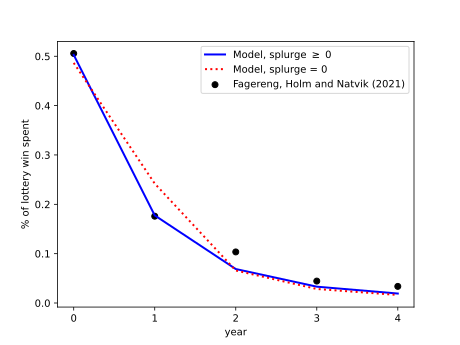
\includegraphics[width=\linewidth]{\econtexRoot/Code/HA-Models/Target_AggMPCX_LiquWealth/Figures/AggMPC_LotteryWin_comparison}
    \caption{Share of lottery win spent}
    \notinsubfile{\label{fig:aggmpclotterywin}}
  \end{subfigure}
  \begin{subfigure}[b]{.48\linewidth}
    \centering
    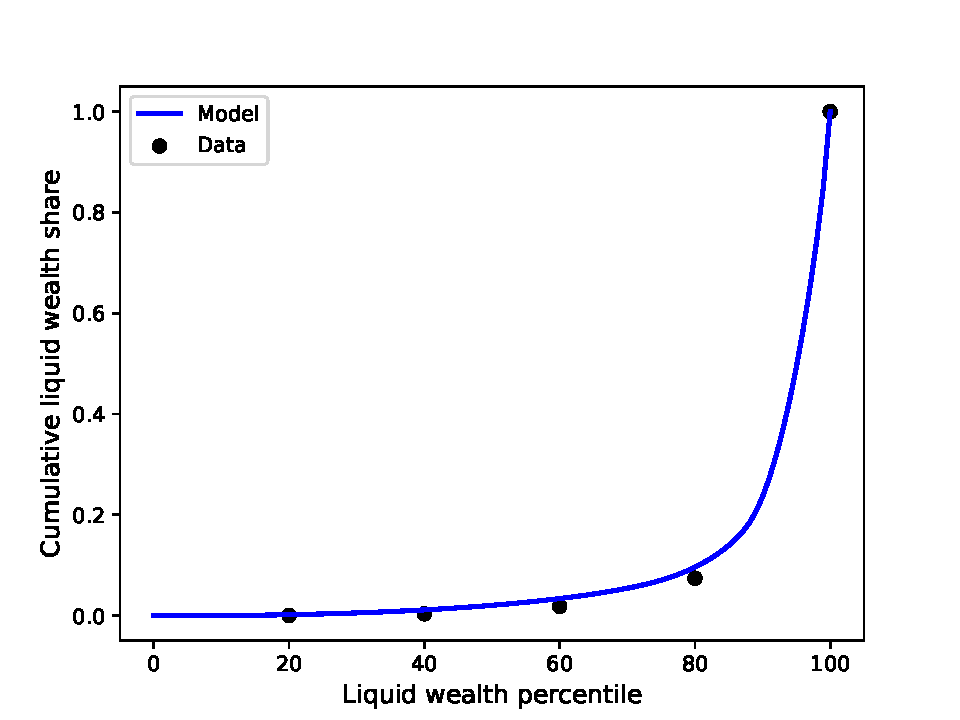
\includegraphics[width=\linewidth]{\econtexRoot/Code/HA-Models/Target_AggMPCX_LiquWealth/Figures/LiquWealth_Distribution_comparison}
    \caption{Distribution of liquid wealth}
    \notinsubfile{\label{fig:liquwealthdistribution}}
  \end{subfigure}%
  \caption{Marginal propensity to consume over time and the liquid wealth distribution in the model and the data}
  \notinsubfile{\label{fig:splurge_estimation}}
  \parbox{16cm}{\small \vspace{.15cm} \textbf{Note}: Panel (a) shows the fit of the model to the dynamic consumption response estimated in \citet{fagereng_mpc_2021}; see their figure~A5.
Panel (b) shows the fit of the model to the distribution of liquid wealth (see Section~\ref{sec:SCFdata} for the definition) from the 2004 SCF.\normalsize}
\end{figure}


% \newcommand{\iMPC}{\econtexRoot/Code/HA-Models/Target_AggMPCX_LiquWealth/Figures/AggMPC_LotteryWin_comparison}
% \newcommand{\LiqDist}{\econtexRoot/Code/HA-Models/Target_AggMPCX_LiquWealth/Figures/LiquWealth_Distribution_comparison}
% \begin{figure}[htb]
%   \ifdefined\HCode
%     \HCode{<div style="text-align: center;">}
%   \fi
%   \centering
%   \begin{tabular*}{\textwidth}{@{\extracolsep{\fill}}cc@{}}
%     \ifdefined\HCode
%       \HCode{<div style="display: flex; flex-direction: column; align-items: center; width: 48\%;">}
%     \fi
%     \subfloat[Share of lottery win spent\label{fig:aggmpclotterywin}]{%
%       \ifdefined\HCode
%         \includegraphics[width=\linewidth]{\iMPC}
%       \else
%         \includegraphics[width=0.48\textwidth]{\iMPC}
%       \fi
%     }
%     \ifdefined\HCode
%       \HCode{</div>}
%     \fi
%     &
%     \ifdefined\HCode
%       \HCode{<div style="display: flex; flex-direction: column; align-items: center; width: 48\%;">}
%     \fi
%     \subfloat[Distribution of liquid wealth\label{fig:liquwealthdistribution}]{%
%       \ifdefined\HCode
%         \includegraphics[width=\linewidth]{\LiqDist}
%       \else
%         \includegraphics[width=0.48\textwidth]{\LiqDist}
%       \fi
%     }
%     \ifdefined\HCode
%       \HCode{</div>}
%     \fi
%   \end{tabular*}
%   \ifdefined\HCode
%     \HCode{<figcaption style="text-align: center; width: auto; max-width: 800px;">}
%   \fi
%   \caption{Targets and model moments from the estimation}
%   \notinsubfile{\label{fig:splurge_estimation}}
%   \ifdefined\HCode
%     \HCode{<div style="text-align: justify; width: 16cm;  margin: 1em auto 0 auto;">}
%   \fi

% \parbox{14cm}{
%   \footnotesize \vspace{.15cm} Panel (a) shows the fit of the model to the dynamic consumption response estimated in \citet{fagereng_mpc_2021}; see their figure~A5. Panel (b) shows the fit of the model to the distribution of liquid wealth (see Section~\ref{sec:SCFdata} for the definition) from the 2004 SCF.\normalsize}
% \end{figure}

\begin{table}[t]
  \center
  \begin{tabular}{@{}lcccccc@{}} 
\toprule 
                  & \multicolumn{5}{c}{MPC} &   \\   
                  &  1st WQ  & 2nd WQ  & 3rd WQ & 4th WQ  & Agg  &  K/Y  \\  \midrule 
Model &0.27 & 0.49 & 0.60 & 0.66 & 0.50 & 6.59 \\ 
Data &0.39 & 0.39 & 0.55 & 0.66 & 0.51 & 6.60 \\ \bottomrule
\end{tabular}  

  \caption{Marginal propensities to consume across wealth quartiles and the total population as well as the wealth to income ratio, in the model and according to the data}
  \notinsubfile{\label{tab:MPC_WQ}}
\end{table}


For this estimation exercise, the remaining model parameters are calibrated to reflect the Norwegian economy.
Specifically, we set the real interest rate to $2$ percent annually and the unemployment rate to $4.4$ percent, in line with \citet{aursland_state-dependent_2020}.
The quarterly probability to survive is calibrated to $1-1/160$, reflecting an expected working life of 40 years.
Aggregate productivity growth is set to $1$ percent annually, following \citet{kravik_navigating_2019}.
The unemployment net replacement rate is calibrated to $60$ percent, following \citet{oecd_net_2020}.
Finally, we set the real interest rate on liquid debt to $13.6$ percent, following data from the Norwegian debt registry \citet{gjeldsregistret_nokkeltall_2022}.\footnote{Specifically, we determine the average volume-weighted interest rate on liquid debt, which consists of consumer loans, credit and payment card debt and all other unsecured debt.
We use data from December 2019.
Note that although these data let us pin down aggregate quantities, they do not solve the issue referred to in footnote~\ref{foot:liqwealth}, since we cannot link them to the tax registry at the individual level.
We set the borrowing limit on liquid debt to zero.}

Estimates of the standard deviations of the permanent and transitory shocks are taken from \citet{crawley2024parsimonious}, who estimate an income process on administrative data for Norwegian males from 1971 to 2014.
The estimated annual variances for the permanent and transitory shocks are 0.004 and 0.033, respectively.\footnote{As shown in \citet{crawley2024parsimonious}, an income process of the form that we use here is more accurately estimated using moments in levels not differences.
Hence, we take the numbers from column 3 of Panel C in their table 4.} As in \citet{carroll2020sticky}, these are converted to quarterly values by multiplying the permanent and transitory shock variances by $1/4$ and $4$, respectively.
Thus, we obtain quarterly standard deviations of $\sigma_\psi=0.0316$ and $\sigma_\xi=0.363$.

Using the calibrated model, we simulated unexpected lottery winnings and calculate the share of the lottery spent in each year.
Specifically, each simulated agent receives a lottery win in a random quarter of the first year of the simulation.
The size of the lottery win is itself random and spans the range of lottery sizes found in \citet{fagereng_mpc_2021}.
The estimation procedure minimizes the distance between the target and model moments by selecting the splurge factor and the distribution of discount factors in the population, where the latter are assumed to be uniformly distributed in the range $[\beta-\nabla, \beta+\nabla]$.
We approximate the uniform distribution of discount factors with a discrete approximation and let the population consist of eight different types.

The estimation yields a splurge factor of $0.249$ and a distribution of discount factors described by $\beta = 0.968$ and $\nabla=0.0578$.
Given these estimated parameters and the remaining calibrated ones, the model is able to replicate the time path of consumption in response to a lottery win from \citet{fagereng_mpc_2021} and the targeted distribution of liquid wealth very well, see Figure \ref{fig:splurge_estimation}.
Also, the targeted moments discussed in Table \ref{tab:MPC_WQ} are captured relatively well.
In particular, the model is able to account for the empirical fact that MPC consume for high-wealth agents is substantially larger than zero, see the first column.




 

\hypertarget{data-on-permanent-income-liquid-wealth-and-education}{}\par\subsection{Data on permanent income, liquid wealth, and education}
\notinsubfile{\label{sec:SCFdata}}

Before we move on to the parameterization of the full model, we describe in detail the data that we use to get measures of permanent income, liquid wealth, and the division of households into educational groups in the United States.
We use data on the distribution of liquid wealth from the 2004 wave of the SCF.
We restrict our attention to households where the head is of working age, which we define to be in the range from 25 to 62.
The SCF-variable ``normal annual income'' is our measure of the household's permanent income, and, to exclude outliers, we drop the observations that make up the bottom 5 percent of the distribution of this variable.
The smallest value of permanent income for households in our sample is thus \$16,708.


Liquid wealth is defined as in \cite{kaplan2014model} and consists of cash, money market, checking, savings, and call accounts; directly held mutual funds; and stocks and bonds.
We subtract off liquid debt, which is the revolving debt on credit card balances.
Note that the SCF does not contain information on cash holdings, so these are imputed with the procedure described in Appendix B.1 of \cite{kaplan2014model}, which also describes the credit card balances that are considered part of liquid debt.
We drop any households that have negative liquid wealth.


Households are classified into three educational groups.
The first group, ``Dropout,'' applies to households where the head of household has not obtained a high school diploma; the second group, ``Highschool,'' includes heads of households who have a high school diploma and those who, in addition, have some years of college education without obtaining a bachelor's degree; and the third group, ``College,'' consists of heads of households who have obtained a bachelor's degree or higher.
With this classification of the education groups, the Dropout group makes up $9.3$ percent of the population, the Highschool group $52.7$ percent, and the College group $38.0$ percent.


With our sample selection criteria, we are left with a sample representing about 61.3 million U.S.
households.

\subsection{Parameters in the full model}
\notinsubfile{\label{sec:paramsFull}}

With households classified into the three education groups using the SCF data, we proceed to set the parameters of the model as follows.
First, we calibrate a set of parameters that apply to all types of houesholds in the model.
Second, we calibrate another set of parameters that are specific to each education group to capture broad differences across these groups.
Finally, given the calibrated parameters we estimate discount factor distributions for each education group that allow us to match the distribution of liquid wealth in each group.


The model is a simplified model for households in that we do not take into account heterogeneity across household size or composition.
The households are ex-ante heterogeneous in their subjective discount factors as well as their level of education.
We classify the education level of the household based on the education of the head of the household, and we typically think of individual characteristics as applying to that person.


A period in the model is one quarter.
This choice makes it realistic to consider stimulus policies that are implemented in the same period as a recession starts.


\subsubsection{Calibrated parameters} 
\notinsubfile{\label{sec:calib}}

Panel~A of table~\ref{tab:calibration}, lists parameters that are calibrated equally across all types in the model.
Panel~B of table~\ref{tab:calibration}, lists parameters in the model that are education specific.
For completeness, panel~C of table~\ref{tab:calibration} summarizes the parameters describing how we model a recession and the three policies we consider as potential responses to a recession.


\textbf{Preferences, survival and interest rates.} All households are assumed to have a coefficient of relative risk aversion equal to $\gamma=2$.
We also assume that all households have the same propensity to splurge out of transitory income gains and set $\varsigma=0.249$, the value estimated in section~\ref{sec:splurge}.
However, each education group is divided into types that differ in their subjective discount factors.
The distributions of discount factors for each education group are estimated to fit the distribution of liquid wealth within that group, and this estimation is described in detail in section~\ref{sec:estimBetas}.
Regardless of type, households face a constant survival probability each quarter.
This probability is set to $1-1/160$, reflecting an expected working life of 40 years.
The real interest rate on households' savings is set to $1$ percent per quarter.



\afterpage{
  \thispagestyle{empty}
  \begin{table}[p]
    \caption{Calibrated Model Parameters}
    \center
%    \begin{center}
      \begin{tabular}{c}
        \begin{tabular}{lcd{3}} 
          \toprule
          \multicolumn{3}{l}{Panel (A) Parameters that apply to all types} \\ \midrule
          Parameter & Notation & \text{Value} \\ \midrule 
          Risk aversion & $\gamma$ & 2.0 \\ 
          Splurge & $\varsigma$ & 0.249 \\ 
          Survival probability, quarterly & $1-D$ & 0.994 \\
          Risk free interest rate, quarterly (gross) & $R$ & 1.01 \\ 
          Standard deviation of transitory shock & $\sigma_\xi$ & 0.346 \\
          Standard deviation of permanent shock & $\sigma_\psi$ & 0.0548 \\ 
          Unemployment benefits replacement rate (share of PI) & $\rho_b$ & 0.7 \\ 
          Unemployment income w/o benefits (share of PI) & $\rho_{nb}$ & 0.5 \\ 
          Avg. duration of unemp. benefits in normal times (quarters) & & 2 \\
          Avg. duration of unemp. spell in normal times (quarters) & & 1.5 \\
          Probability of leaving unemployment & $\pi_{ue}$ & 0.667 \\ 
          Consumption elasticity of aggregate demand effect & $\kappa$ & 0.3 
          \\ \bottomrule 
        \end{tabular} \\ \\

        \begin{tabular}{lccc}
          \toprule 
          \multicolumn{4}{l}{Panel (B) Parameters calibrated for each education group} \\ \midrule
          & Dropout & Highschool & College \\ \midrule
          Percent of population & \phantom{0}9.3 & 52.7 & 38.0 \\ 
          Avg. quarterly PI of ``newborn'' agent (\$1000) & \phantom{0}6.2 & 11.1 & 14.5 \\
          Std. dev. of $\log($PI$)$ of ``newborn'' agent & 0.32 & 0.42 & 0.53 \\
          Avg. quarterly gross growth rate of PI ($\Gamma_e$) & 1.0036 & 1.0045 & 1.0049 \\
          Unemployment rate in normal times (percent) & \phantom{0}8.5 & \phantom{0}4.4 & \phantom{0}2.7 \\ 
          Probability of entering unemployment ($\pi_{eu}^{e}$, percent) & \phantom{0}6.2 & \phantom{0}3.1 & \phantom{0}1.8 
          \\ \bottomrule 
        \end{tabular} \\
        \ifdefined\HCode
        \HCode{<div style="text-align: justify; width: 16cm;  margin: 1em auto 0 auto;">}
        \fi
        \parbox{16cm}{\footnotesize \vspace{.25cm} \textbf{Note}: The first three rows show numbers from the 2004 SCF.
The fourth row are averages of growth rates from \cite{carroll2020modeling}.
The fifth row are numbers for 2004 from the Bureau of Labor Statistics, and the sixth row are calculated from these unemployment rates.\normalsize}
        \\ \\

        \begin{tabular}{lc}
          \toprule 
          \multicolumn{2}{l}{Panel (C) Parameters describing policy experiments} \\ \midrule 
          Parameter & Value \\ \midrule 
          Change in unemployment rates in a recession & $\times 2$ \\ 
          Expected unemployment spell in a recession & 4 quarters \\ 
          Average length of recession & 6 quarters \\ 
          Size of stimulus check & \$1,200 \\ 
          PI threshold for reducing check size & \$100,000 \\ 
          PI threshold for not receiving check & \$150,000 \\ 
          Extended unemployment benefits & 4 quarters \\
          Length of payroll tax cut & 8 quarters \\ 
          Income increase from payroll tax cut & 2 percent \\ 
          Belief (probability) that tax cut is extended & 50 percent 		
          \\ \bottomrule
        \end{tabular} 

      \end{tabular}
%    \end{center}
    \begin{tabular}{p{16cm}}
%      \parbox{16cm}{
      \medskip
      \small Panel (A) shows parameters calibrated the same for all types. Panel (B) shows parameters calibrated for each education group. Panel (C) shows the numbers describing how we model a recession and the three policies we consider. ``PI'' refers to permanent income.
      % }
      \end{tabular}
    \notinsubfile{\label{tab:calibration}}
  \end{table}
  \clearpage
}

\textbf{Labor market risk while employed.} When consumers are born, they receive an initial level of permanent income.
This initial value is drawn from a log-normal distribution that depends on the education level the household is born with.
For each education group, the parameters of the distribution are determined by the mean and standard deviation of log-permanent income for households in that group where the head of the household is of age 25 in the SCF 2004.
For the Dropout group, the mean initial value of quarterly permanent income is \$6,200; for the Highschool group, it is \$11,100; and for the College group, it is \$14,500.
The standard deviations of the log-normal distributions for each group are, respectively, $0.32$, $0.42$, and $0.53$.


While households remain employed, their income is subject to both permanent and transitory idiosyncratic shocks.
These shocks are distributed equally for the three education groups.
The standard deviations of these shocks are taken from \cite{carroll2020sticky}, who set the standard deviations of the transitory and permanent shocks to $\sigma_\xi=0.346$ and $\sigma_\psi=0.0548$, respectively.


Permanent income also grows, on average, with a growth rate $\Gamma_{e(i)}$ that depends on the level of education.
These average growth rates are based on numbers from \cite{carroll2020modeling}, who construct age-dependent expected permanent income growth factors using numbers from \cite{cagetti2003wealth} and fit the age-dependent numbers to their life-cycle model.
We construct the quarterly growth rates of permanent income in our perpetual-youth model by taking the average of the age-dependent growth rates during a household's working life.
The average gross quarterly growth rates that we obtain for the three education groups are then $\Gamma_d=1.0036$, $\Gamma_h=1.0045$, and $\Gamma_c=1.0049$.

\textbf{Unemployment.} Consumers also face the risk of becoming unemployed and will then have access to unemployment benefits for a certain period.
The parameters describing the unemployment benefits in normal times are based on the work of \cite{rothstein2017scraping}, who study the effects on household income of unemployment and of running out of eligibility for benefits.
The unemployment benefits replacement rate is thus set to $\rho_b=0.7$ for all households, and when benefits run out, the unemployment replacement rate without any benefits is set to $\rho_{nb}=0.5$.
These replacement rates are set as a share of the households' permanent income and are based on the initial drop in income upon entering an unemployment spell, presented in figure~3 in \cite{rothstein2017scraping}.\footnote{See the lines for their UI exhaustee sample including and excluding UI income.
\cite{rothstein2017scraping} also point out that ``UI benefits replace about 40 percent of the lost earnings on average'' (page 894).
For a household with two income earners with equal income, these findings would mean that income drops to 70 percent when one earner becomes unemployed and to 50 percent when benefits run out.
In this paper we ignore several of the channels studied by \cite{rothstein2017scraping} such as within household insurance and other social programs that can provide income even after UI benefits have run out.} 

The duration of unemployment benefits in normal times is set to two quarters, so that our Markov transition matrix $\Pi$ has four states.
This length of time corresponds to the mean duration of unemployment benefits across U.S.
states from 2004 to mid-2008 of 26 weeks, reported by \cite{rothstein2017scraping}.


The probability of transitioning out of unemployment is set to match the average duration of an unemployment spell in normal times.
In data from the Bureau of Labor Statistics, this average duration was 19.6 weeks or 1.5 quarters in 2004.
We do not have data on  education-specific duration rates, however, so we set the average duration of unemployment to 1.5 quarters for all households.
This implies that the transition probability from unemployment to employment is set to $\pi_{ue}=2/3$.


The Bureau of Labor Statistics provide data on unemployment rates for different education groups, and we match the average rate in each group in 2004 by setting an education-specific probability of transitioning from employment into unemployment.
Note that this calibration strategy is consistent with the results in \citet{mincer1991education} who finds that the main difference between education groups is in the incidence of unemployment, and not its duration.\footnote{\citet{mincer1991education} states that ``the reduction of the incidence of unemployment [at higher education levels] is found to be far more important than the reduced duration of unemployment in creating the educational differentials in unemployment rates'' (page 1).} More recent work by \citet{elsby2010labor} includes data upto 2009 and echoes \citeauthor{mincer1991education}'s results.


The average unemployment rate in 2004 was 8.5 percent for the Dropout group, 4.4 percent for the Highschool group, and 2.7 percent for the College group.
These values imply that the probabilities of transitioning into unemployment in normal times are $\pi_{eu}^d=6.2$ percent, $\pi_{eu}^h=3.1$ percent, and $\pi_{eu}^c=1.8$ percent, respectively.\footnote{Also note that the probability of transitioning from employment to unemployment is the probability of a job separation times the conditional probability of unemployment given a job separation.
\citet{mincer1991education} reports that both of these are lower for higher education levels.
For our calibration, this means that a higher job finding rate \textit{within} the quarter of the job separation for more educated workers translates	into a lower probability of transitioning from employment to unemployment during a quarter.
In that sense, our calibration is consistent with short-term job-finding rates being higher for more educated workers.}

Finally, the strength of the aggregate demand effect in recessions is determined by the consumption elasticity of productivity.
We follow \cite{kmpHandbook2016} and set this to $\kappa=0.3$.



\hypertarget{estimating-the-discount-factor-distributions}{}\par\subsubsection{Estimating the discount factor distributions} 
\notinsubfile{\label{sec:estimBetas}}

Discount factor distributions are estimated separately for each education group to match the distribution of liquid wealth for households in that group.
To do so, we let each education group consist of types that differ in their subjective discount factor,~$\beta$.
The discount factors within each group $e\in \{d, h, c\}$ are assumed to be uniformly distributed in the range $[\beta_e-\nabla_e, \beta_e+\nabla_e]$.
The parameters $\beta_e$ and $\nabla_e$ are chosen for each group separately to match the median liquid-wealth-to-permanent-income ratio and the $\nth{20}$, $\nth{40}$, $\nth{60}$, and $\nth{80}$ percentile points of the Lorenz curve for liquid wealth for that group.
We approximate the uniform distribution of discount factors with a discrete approximation and let each education group consist of seven different types.

Panel~A of table~\ref{tab:estimBetas} shows the estimated values of $(\beta_e, \nabla_e)$ for each education group.
The panel also shows the minimum and maximum values of the discount factors we actually use in the model when we use a discrete approximation with seven values to approximate the uniform distribution of discount factors.
Panel~B of table~\ref{tab:estimBetas} shows that with these estimated distributions, we can exactly match the median liquid-wealth-to-permanent-income ratios for each education group.
Figure~\ref{fig:LorenzPts} shows that with the estimated distributions, the model quite closely matches the distribution of liquid wealth within each education group as well as for the population as a whole.
Thus, our model does not suffer from the ``missing middle'' problem, identified in \cite{kaplanMPC2022}, in which the middle of the wealth distribution has too little wealth.

%Our model avoids this problem for two reasons: (1) The splurge pushes up MPCs relative to wealth, and (2) we calibrate to liquid wealth rather than total wealth.

\begin{table}[th]
  \begin{center}
    \begin{tabular}{l}
      \begin{tabular}{lccc}
        \multicolumn{4}{l}{Panel (A) Estimated discount factor distributions} \\ \midrule
        & Dropout & Highschool & College \\ \midrule
        $(\beta_e, \nabla_e)$ & (0.719, 0.318) & (0.911, 0.137) & (0.983, 0.014) \\
        (Min, max) in approximation & (0.447, 0.991) & (0.793, $0.990^*$) & (0.971, 0.995) \\
        \midrule 
      \end{tabular} \\ \\ 
      
      \begin{tabular}{lccc}
        \multicolumn{4}{l}{Panel (B) Estimation targets} \\ \midrule
        & Dropout & Highschool & College \\ \midrule
        Median LW/ quarterly PI (data, percent) & 4.64 & 30.2 & 112.8 \\ 
        Median LW/ quarterly PI (model, percent) & 4.64 & 30.2 & 112.8 %\\
        %         $[20,40,60,80]$ pctiles of Lorenz curve (data) & $[0, 0.01, 0.6, 3.6]$ & $[0.06, 0.6, 3.0, 11.6]$ & $[0.2, 0.9, 3.3, 10.3]$ \\
        %         $[20,40,60,80]$ pctiles of Lorenz curve (model) & $[0.0, 0.0, 0.6, 3.6]$ & $[0.05, 0.8, 3.1, 11.5]$ & $[0.3, 1.3, 3.6, 10.1]$
        \\ \midrule 
      \end{tabular} \\ \\ 
    \end{tabular}
    \caption{Estimated discount factor distributions and estimation targets}
    \notinsubfile{\label{tab:estimBetas}}
    \parbox{16cm}{\small \vspace{.15cm} \textbf{Note}: Panel (A) shows the estimated parameters of the discount distributions for each education group.
It also shows the minimum and maximum values we use in our discrete approximation to the uniform distribution of discount factors for each group.
The $*$ indicates that the highest value in the uniform distribution of discount factor values violates the growth impatience condition (GIC) and has been replaced.
Panel (B) shows the weighted median ratio of liquid wealth to permanent income from the 2004 SCF and in the model.
In the annual data from the SCF, the annual PI is divided by 4 to obtain a quarterly number.\normalsize}
  \end{center}
\end{table}

One point we should note concerns the estimated discount factor distribution for the Highschool group.
Panel~A of table~\ref{tab:estimBetas} reports values of $\beta_h=0.911$ and $\nabla_h=0.137$.
With these values, the largest discount factors in our discrete approximation of the uniform distribution in the range $[\beta_h-\nabla_h, \beta_h+\nabla_h]$ would be greater than $1$.
More importantly, the value would violate the Growth Impatience Condition (GIC), discussed in \cite{carroll2022theoretical}.
(The GIC is required to prevent the ratio of total wealth to total income of any group from approaching infinity.
It does this by making sure that the growth of wealth of the group is less than or equal to the growth of income.)
We replace values violating the GIC with values close to the upper bound on $\beta$ imposed by the GIC.
In panel~A of table~\ref{tab:estimBetas} the largest value is marked by a $*$ to indicate that it has been replaced to avoid violating the GIC.
We always impose that the GIC is satisfied in the estimation of the discount factor distributions, but for the baseline parameter values it is only binding for the Highschool group.
Thus, the estimation can select a large value of $\nabla_h$ without violating the constraint.\footnote{The constraint is imposed by calculating a discount factor $\beta^{\text{GIC}}$ where the GIC holds with equality.
Then the estimation can pick how close to this value the largest discount factor is by estimating $x$ and setting the largest discount factor to $\exp(x)/(1+\exp(x)) \beta^{\text{GIC}}$.} 

\begin{figure}[th]
  \begin{center}
    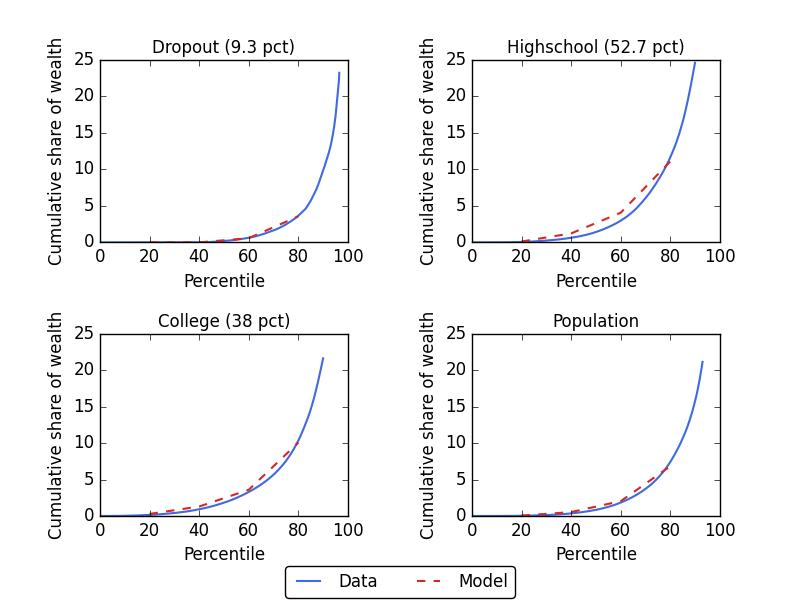
\includegraphics[width=.9\textwidth]{\econtexRoot/Figures/LorenzPoints_CRRA_2.0_R_1.01}
    \caption{Distributions of liquid wealth within each education group and for the whole population from the 2004 Survey of Consumer Finances and from the model with estimated discount factor distributions}
    \notinsubfile{\label{fig:LorenzPts}}
    \parbox{16cm}{\small \vspace{.15cm} \textbf{Note}: The discount factor distributions are estimated separately for each education group to fit the median liquid-wealth-to-permanent-income ratio and the $\nth{20}$, $\nth{40}$, $\nth{60}$, and $\nth{80}$ percentile points of the Lorenz curve for liquid wealth for that group. The ``Population'' panel compares the wealth distribution that results from pooling the three groups in the model to the overall wealth distribution in the data.\normalsize}
  \end{center}
\end{figure}

Also, note that several of the types in the Dropout group have very low discount factors and are very impatient.
In this way, the model fits the feature of the data for the Dropout group that the bottom quintiles do not save at all and do not accumulate any liquid wealth.
Very low estimates for discount factors are in line with those obtained in the literature on payday lending.\footnote{See, for example, \cite{skiba2008payday}, who estimate two-week discount rates of $21$ percent, and \cite{allcott2021high}, who estimate an initial period discount factor between $0.74$ and $0.83$ in a model where a period is eight weeks long.
Both of these papers use quasi-hyperbolic preferences, so the estimates are not directly comparable with parameters in our model.
Nevertheless, they support the point that very high discount rates are necessary to model the part of the population that takes out payday loans at very high interest rates.} 

\hypertarget{non-targeted-moments}{}\par\subsubsection{Implications for non-targeted moments} 
\notinsubfile{\label{sec:nonTargetedMoments}}

Before we move on to compare different consumption stimulus policies in the calibrated model, we also report implications of the model for some non-targeted moments.
Panel~A of table~\ref{tab:nonTargetedMoments} shows the wealth distribution across the three education groups in the data and in the model.
The model matches these shares quite closely, which may not be surprising given that we calibrate the size of each group and we manage to fit the wealth distribution within each group separately.
The panel also reports the average marginal propensity to consume for the different groups.
To be comparable to numbers reported in \citet{fagereng_mpc_2021}, these are calculated as the average MPC in the year of a lottery win.
Lottery wins occur in a random quarter of the year that differs across individuals.
The MPC for an individual depends on the spending pattern after the win, and these are averaged across individuals within each education group.


Panel~B of table~\ref{tab:nonTargetedMoments} shows similar numbers to Panel~A, sorted by quartiles of the liquid wealth distribution instead of education groups.
Our model yields a slightly more concentrated liquid wealth distribution than in the data.
However, it does produce a fairly high MPC even for households in the highest quartile of the liquid wealth distribution.
This is consistent with the results found in the Norwegian data by \citet{fagereng_mpc_2021}, but also with recent results in \citet{graham2024mental}.
In an administrative dataset from a large US financial institution, they find that the spending response to an income receipt is large across the distribution of liquid asset holdings.
In our model, we obtain this result due to the inclusion of the splurge factor.
As shown in Appendix~\ref{app:Model_without_splurge}, the model is not able to generate a high MPC for the highest wealth quartile without splurge consumption.


\begin{table}[th]
    \centering
    \begin{tabular*}{\textwidth}{@{\extracolsep{\fill}}c@{}}
        \begin{tabular}{lcccc}
            \multicolumn{5}{c}{Panel (A) Non-targeted moments by education group} \\ \midrule
            & Dropout & Highschool & College & Population \\ \midrule
            Percent of liquid wealth (data) & 0.8 & 17.9 & 81.2 & 100 \\
            Percent of liquid wealth (model) & 1.1 & 21.9 & 77.0 & 100 \\
            \makecell[l]{Avg. lottery-win-year MPC \\ (model, incl. splurge)} & 0.78 & 0.61 & 0.38 & 0.54
            \\ \bottomrule 
        \end{tabular} \\ \\

      \vspace{2em}
      
        \begin{tabular}{lcccc}
            \multicolumn{5}{c}{Panel (B) Non-targeted moments by wealth quartile} \\ \midrule
             & WQ 4 & WQ 3 & WQ 2 & WQ 1 \\ \midrule
            Percent of liquid wealth (data) & 0.14 & 1.60 & 8.51 & 89.76 \\
            Percent of liquid wealth (model) & 0.09 & 0.96 & 4.55 & 94.40 \\
            \makecell[l]{Avg. lottery-win-year MPC \\ (model, incl. splurge)} & 0.78 & 0.63 & 0.44 & 0.31
            \\ \bottomrule 
        \end{tabular}
    \end{tabular*}
    \caption{Model fit with respect to non-targeted moments}
    \notinsubfile{\label{tab:nonTargetedMoments}}
    \parbox{16cm}{\small \vspace{.15cm} \textbf{Note}: Panel (A) shows percent of liquid wealth held by each education group in the 2004 SCF and in the model.
It also shows the average MPCs after a lottery win for each education group.
The MPCs are calculated for each individual for the year of a lottery win, taking into account that the win takes place in a random quarter of the year that differs across individuals.
The MPCs are averaged across individuals within each education group.
Panel~(B) shows the same numbers for the population sorted into different quartiles of the liquid wealth distribution.\normalsize}
  \end{table}
  
% \begin{table}[th]
% 	\begin{center}
% 		\begin{tabular}{l}
% 			\begin{tabular}{lcccc}
% 				\multicolumn{5}{l}{Panel (A) Non-targeted moments by education group} \\ \midrule
% 				& Dropout & Highschool & College & Population \\ \midrule
% 				Percent of liquid wealth (data) & 0.8 & 17.9 & 81.2 & 100 \\
% 				Percent of liquid wealth (model) & 1.1 & 21.9 & 77.0 & 100 \\
% 				\makecell[l]{Avg. lottery-win-year MPC \\ (model, incl. splurge)} & 0.78 & 0.61 & 0.38 & 0.54
% 				\\ \bottomrule 
% 			\end{tabular} \\ \\ 
			
% 			\begin{tabular}{lcccc}
% 				\multicolumn{5}{l}{Panel (B) Non-targeted moments by wealth quartile} \\ \midrule
% 				 & WQ 4 & WQ 3 & WQ 2 & WQ 1 \\ \midrule
% 				Percent of liquid wealth (data) & 0.14 & 1.60 & 8.51 & 89.76 \\
% 				Percent of liquid wealth (model) & 0.09 & 0.96 & 4.55 & 94.40 \\
% 				\makecell[l]{Avg. lottery-win-year MPC \\ (model, incl. splurge)} & 0.78 & 0.63 & 0.44 & 0.31
% 				\\ \bottomrule 
% 			\end{tabular}
% 		\end{tabular}
% 		\caption{Implications for non-targeted moments}
% 		\notinsubfile{\label{tab:nonTargetedMoments}}
% 		\parbox{16cm}{\small \vspace{.15cm} \textbf{Note}: Panel (A) shows percent of liquid wealth held by each education group in the 2004 SCF and in the model. It also shows the average MPCs after a lottery win for each education group. The MPCs are calculated for each individual for the year of a lottery win, taking into account that the win takes place in a random quarter of the year that differs across individuals. The MPCs are averaged across individuals within each education group. Panel~(B) shows the same numbers for the population sorted into different quartiles of the liquid wealth distribution.\normalsize}
% 	\end{center}
% \end{table}

Finally, we consider the implications of our model for two different patterns of spending over time.
The first pattern is the dynamics of spending after a lottery win from \citeauthor{fagereng_mpc_2021}.
This pattern was used in the estimation of the splurge factor in section~\ref{sec:splurge}, but was not targeted when estimating the discount factor distributions for each education group in section~\ref{sec:estimBetas}.
Figure~\ref{fig:USaggmpclotterywin} shows that the model that is estimated taking the value of the splurge as given, results in a distribution of spending over time that is very similar to the one found in the Norwegian data.


The second pattern concerns the dynamics of income and spending for households that become unemployed and remain unemployed long enough for unemployment benefits to expire.
Figure~\ref{fig:expiryUI} shows the pattern of income and spending for such households.
\citet{ganongConsumer2019} report the empirical result that nondurable spending drops by 12 percent the month when benefits expire.
Our quarterly model is broadly consistent with this, and the drop in spending the quarter after the expiry of UI benefits is 18 percent.


% \begin{figure}[htb]
%     \centering
%     \begin{minipage}[b]{.48\linewidth}
%         \centering
%         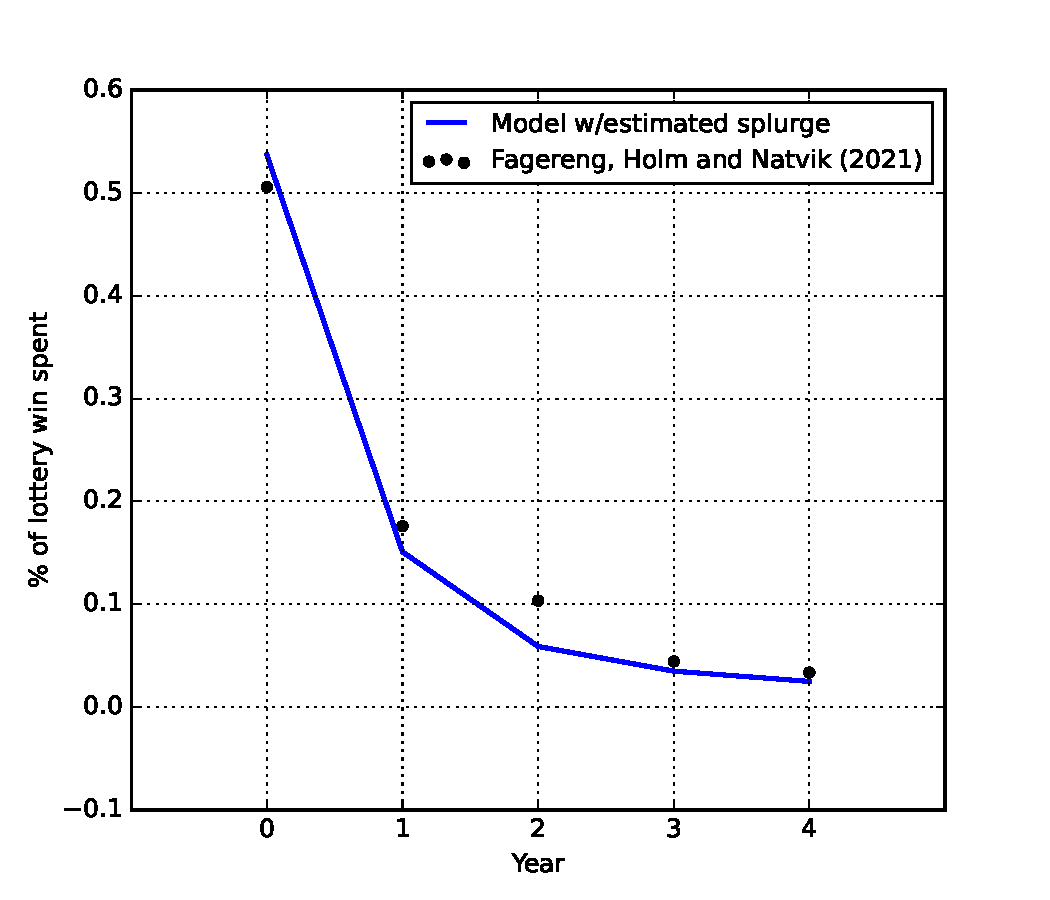
\includegraphics[width=\linewidth]{\econtexRoot/Figures/IMPCs_wSplEstimated}
%         \caption{Share of lottery win spent}
%         \notinsubfile{\label{fig:USaggmpclotterywin}}
%     \end{minipage}%
%     \hfill
%     \begin{minipage}[b]{.48\linewidth}
%         \centering
%         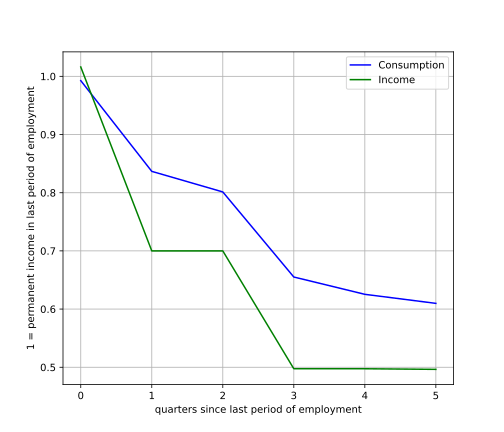
\includegraphics[width=\linewidth]{\econtexRoot/Code/HA-Models/FromPandemicCode/Figures/UnempSpell_Dynamics}
%         \caption{Spending upon expiry of UI benefits}
%         \notinsubfile{\label{fig:expiryUI}}
%     \end{minipage}
%     \caption{Untargeted moments}
%     \notinsubfile{\label{fig:untargetedMoments}}
%     \parbox{16cm}{\small \vspace{.15cm} \textbf{Note}: Panel (a) compares the dynamic consumption response in the model to the estimates in \citet{fagereng_mpc_2021}; see their Figure~A5. Panel (b) shows the evolution of income and spending for households who remain unemployed long enough for UI benefits to expire; see Figure~2 in \citet{ganongConsumer2019}.\normalsize}
% \end{figure}

\begin{figure}[htb]
    \centering
    \begin{subfigure}[b]{.48\linewidth}
        \centering
        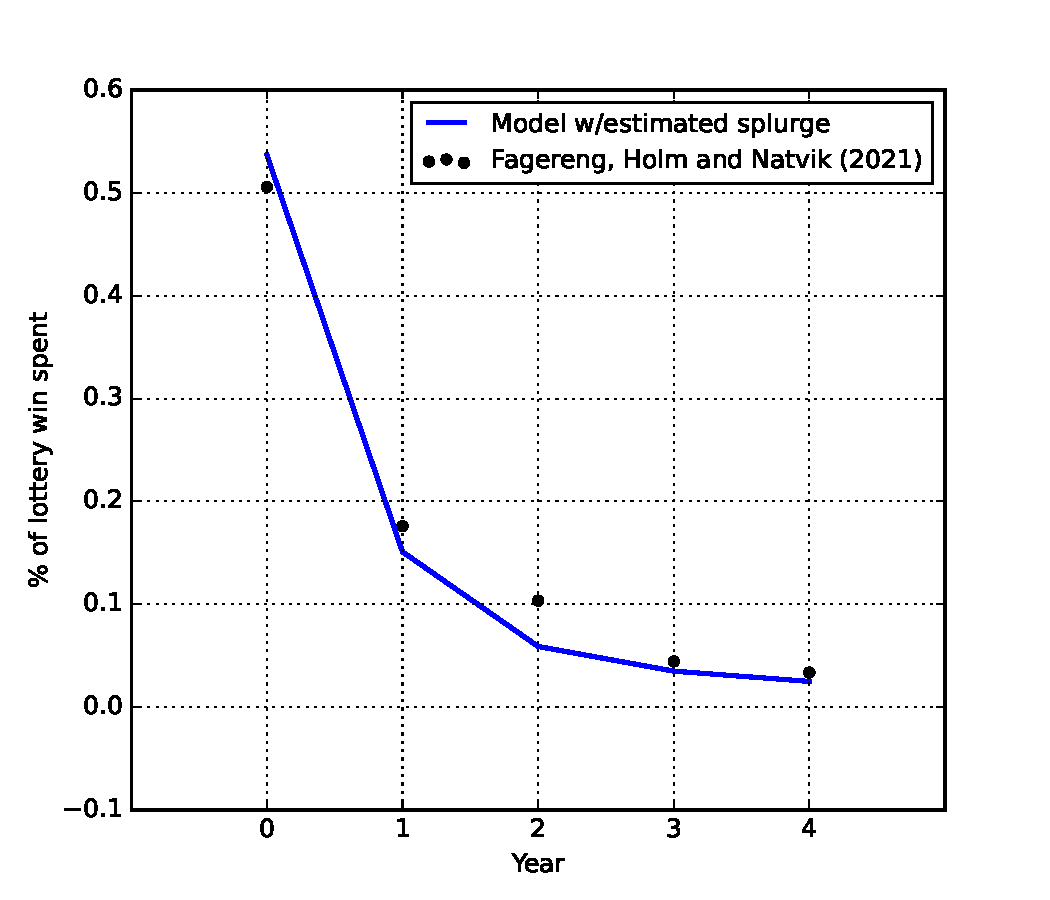
\includegraphics[width=\linewidth]{\econtexRoot/Figures/IMPCs_wSplEstimated}
        \caption{Share of lottery win spent}
        \notinsubfile{\label{fig:USaggmpclotterywin}}
    \end{subfigure}%
    \begin{subfigure}[b]{.48\linewidth}
        \centering
        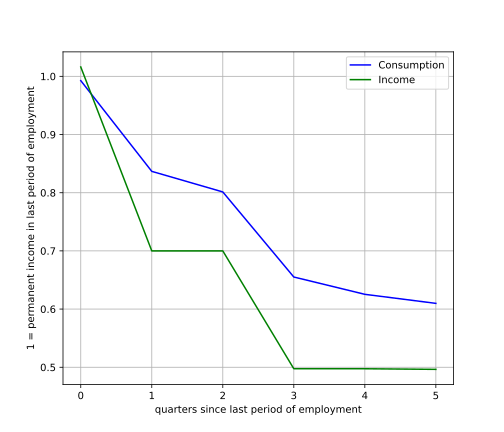
\includegraphics[width=\linewidth]{\econtexRoot/Code/HA-Models/FromPandemicCode/Figures/UnempSpell_Dynamics}
        \caption{Spending upon expiry of UI benefits}
        \notinsubfile{\label{fig:expiryUI}}
    \end{subfigure}
    \caption{Marginal propensity to consume over time and the spending upon expiry of UI benefits in the model}
    \notinsubfile{\label{fig:untargetedMoments}}
    \parbox{16cm}{\small \vspace{.15cm} \textbf{Note}: Panel (a) compares the dynamic consumption response in the model to the estimates in \citet{fagereng_mpc_2021}; see their Figure~A5.
Panel (b) shows the evolution of income and spending for households who remain unemployed long enough for UI benefits to expire; see Figure~2 in \citet{ganongConsumer2019}.\normalsize}
  \end{figure}
  
% \begin{figure}[htb]
%   \ifdefined\HCode
%     \HCode{<div style="text-align: center;">}
%   \fi
%   \centering
%   \begin{tabular*}{\textwidth}{@{\extracolsep{\fill}}cc@{}}
%     \ifdefined\HCode
%       \HCode{<div style="display: flex; flex-direction: column; align-items: center; width: 48\%;">}
%     \fi
%     \subfloat[Share of lottery win spent\label{fig:USaggmpclotterywin}]{%
%       \ifdefined\HCode
%         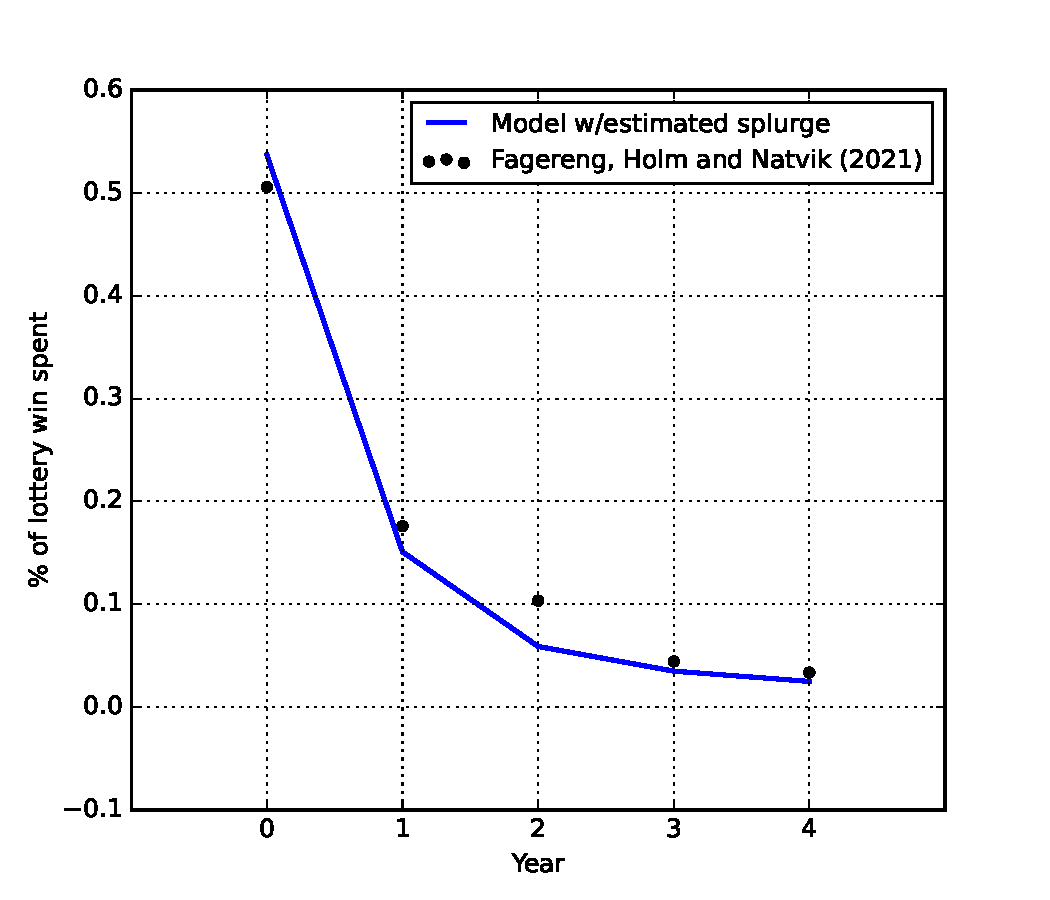
\includegraphics[width=\linewidth]{\econtexRoot/Figures/IMPCs_wSplEstimated}
%       \else
%         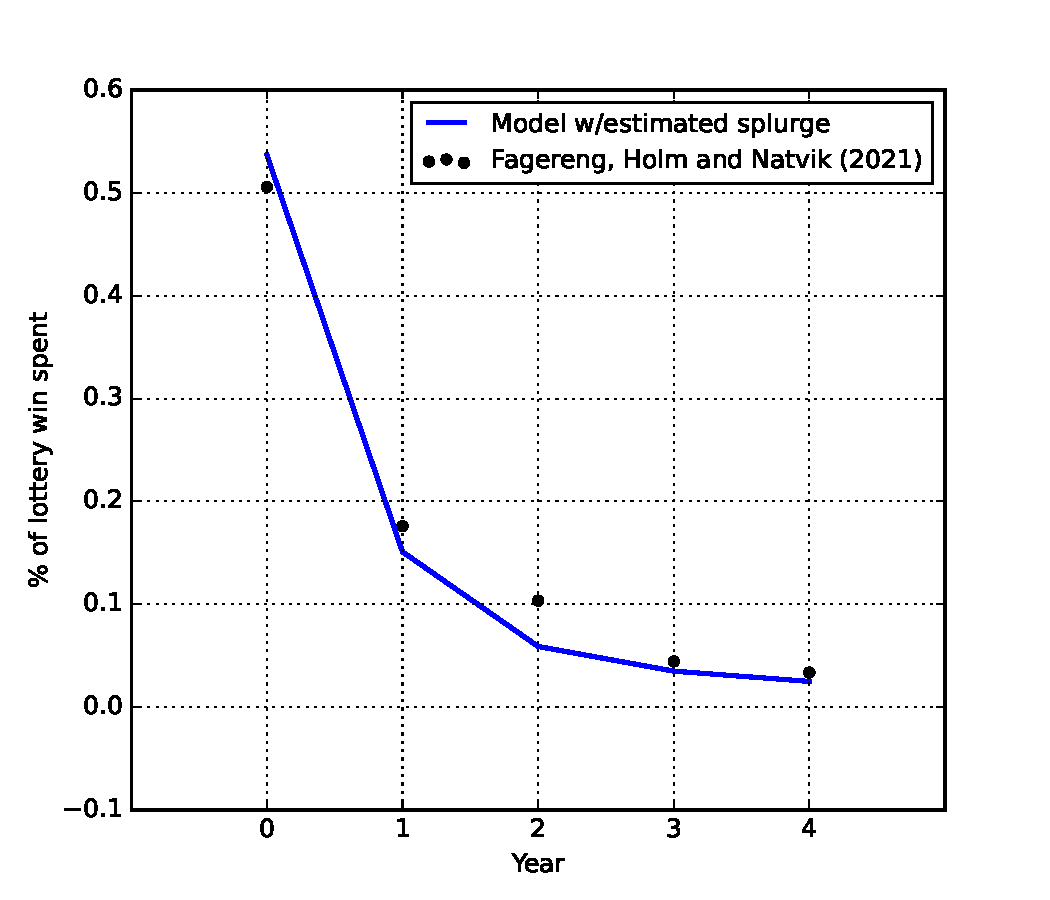
\includegraphics[width=0.48\textwidth]{\econtexRoot/Figures/IMPCs_wSplEstimated}
%       \fi
%     }
%     \ifdefined\HCode
%       \HCode{</div>}
%     \fi
%     &
%     \ifdefined\HCode
%       \HCode{<div style="display: flex; flex-direction: column; align-items: center; width: 48\%;">}
%     \fi
%     \subfloat[Spending upon expiry of UI benefits\label{fig:expiryUI}]{%
%       \ifdefined\HCode
%         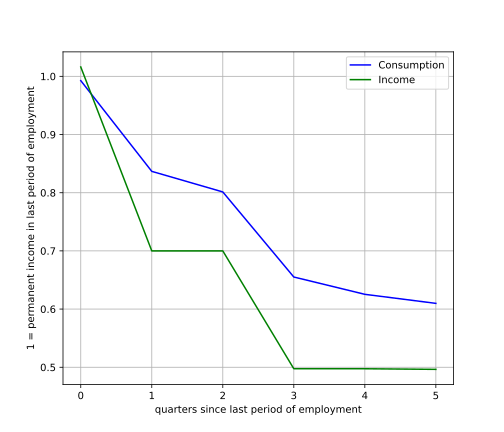
\includegraphics[width=\linewidth]{\econtexRoot/Code/HA-Models/FromPandemicCode/Figures/UnempSpell_Dynamics}
%       \else
%         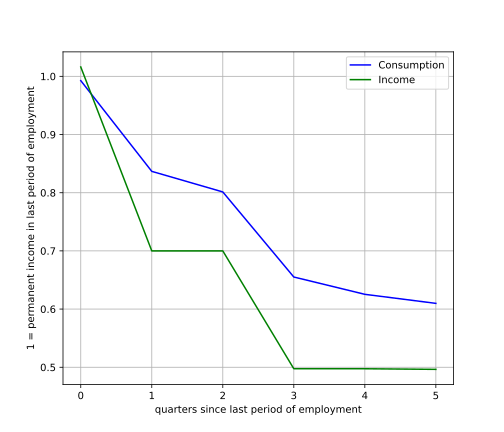
\includegraphics[width=0.48\textwidth]{\econtexRoot/Code/HA-Models/FromPandemicCode/Figures/UnempSpell_Dynamics}
%       \fi
%     }
%     \ifdefined\HCode
%       \HCode{</div>}
%     \fi
%   \end{tabular*}
%   \ifdefined\HCode
%     \HCode{<figcaption style="text-align: center; width: auto; max-width: 800px;">}
%   \fi
%   \caption{Untargeted moments}
%   \notinsubfile{\label{fig:untargetedMoments}}
%   \ifdefined\HCode
%     \HCode{<div style="text-align: justify; width: 16cm; margin: 1em auto 0 auto;">}
%   \fi
%   \parbox{16cm}{\small \vspace{.15cm} \textbf{Note}: Panel (a) compares the dynamic consumption response in the model to the estimates in \citet{fagereng_mpc_2021}; see their Figure~A5. Panel (b) shows the evolution of income and spending for households who remain unemployed long enough for UI benefits to expire; see Figure~2 in \citet{ganongConsumer2019}.\normalsize}
%   \ifdefined\HCode
%     \HCode{</div>}
%   \fi
%   \ifdefined\HCode
%     \HCode{</figcaption></div>}
%   \fi
% \end{figure}

\ifthenelse{\boolean{Web}}{}{
  \end{document} \endinput
}


